
\newpage

\section{Crystal structure of sodium chloride (NaCl)}
\label{sec:NaCl}


In the following section, we are going to examine the crytsal structure of NaCl. Using the setup described in~\ref{chap:methods} we recieved the measured intensities as function of the angle $2\theta$. The corresponding graph, depicted in fig.~\ref{fig:Peaks}, shows multiple peaks, which result from diffractions at different Miller planes.  

\begin{figure}[ht]
    \centering
    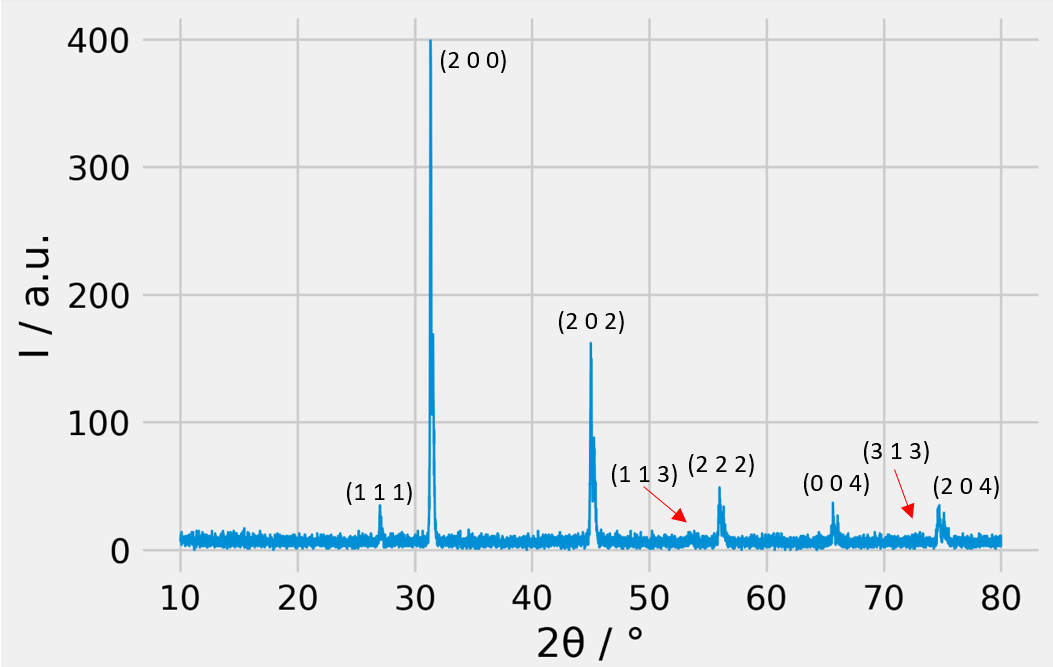
\includegraphics[angle = 90, width = 0.8\linewidth]{Bilder/Auswertung/NaCl/Ivs2thwIndices.png}
    \label{fig:Peaks}
    \caption{The intensity distribution is shown as a function of the angle $2\theta$. The visible and calculated Peaks are labeled with their corresponding Laue indices.}
\end{figure}

It should be noted, that each peak consists of two subpeaks due to the two slightly different wavelengths of the Cu-K$\alpha$1 line and the Cu-K$\alpha$2 line. Therefore, each peak was fitted, but only the values for the Cu-K$\alpha$1 line were taken in account for further calculations. The corresponding values for the full width at half maximum (FWHM) and the intensity of each peak are stated in tab.~\ref{tab:fitVals}.

\begin{table}[ht]
    \centering
    \begin{tabular}{c|c c c}
        \toprule
        Peak No. &  2$\theta_{fit}$ / \SIUnitSymbolDegree &  $I_{fit}$ / a.u. &   FWHM / \SIUnitSymbolDegree \\
        \midrule
            1 &    27.24 &   0.05 &  0.11 \\
            2 &    31.56 &   0.86 &  0.12 \\
            3 &    45.24 &   0.48 &  0.16 \\
            4 &    53.62 &   0.03 &  0.18 \\
            5 &    56.21 &   0.15 &  0.19 \\
            6 &    65.91 &   0.10 &  0.22 \\
            7 &    72.70 &   0.02 &  0.24 \\
            8 &    74.91 &   0.17 &  0.25 \\
        \bottomrule
    \end{tabular}
    \caption{Fit values for each peak in the intensity distribution.}
    \label{tab:fitVals}
\end{table}

Subsequently, the peaks were indexed using the following relations: In order to see a reflex, Bragg's condition 
\begin{equation}
    2 d \sin\theta = m \lambda
    \label{eq411}
\end{equation}
has to be fulfilled. In cubic systems, the distance between to planes $d$ can be calculated simply as 
\begin{equation}
    d_{hkl} = \frac{a^2}{h^2+k^2+l^2}
    \label{eq412}
\end{equation}
with the Laue indices $h$, $k$ and $l$ and the lattice parameter $a$. Using $m=1$ equantions~\ref{eq411} and~\ref{eq:412} can be written together as 
\begin{equation}
    \sin^2\theta = (h^2+k^2+l^2) \frac{\lambda^2}{4a^2}.
\end{equation}
 Here, $c^{-1} := \frac{\lambda^2}{4a^2}$ is a constant parameter depending on the setup. Being reminded, that $(h^2+k^2+l^2) \in \mathbb{N}$ and knowing, that the smallest $2\theta$ is corresponding to small Laue indices, one can assign $h$,$k$,$l$ to $2\theta$, obtaining $a$ from
 \begin{equation}
    a = \sqrt{c}\frac{\lambda}{2}
 \end{equation}
 and $d$ from eq.~\ref{eq412}. All those values can be found in tab.~\ref{tab:latticeParams}.

 \begin{table}
    \centering
    \begin{tabular}{c | c c c c c c c}
        \toprule
        Peak No. &  2$\theta_{fit}$ / \SIUnitSymbolDegree &    d / \SIUnitSymbolAngstrom &  sin2 &  lam2/4a2 &  h2k2l2 &    a / \SIUnitSymbolAngstrom &   h k l \\
        \midrule
        1 &   27.240 & 3.271 & 0.055 &     0.018 &       3 & 5.666 & (1 1 1) \\
        2 &   31.563 & 2.832 & 0.074 &     0.018 &       4 & 5.665 & (0 0 2) \\
        3 &   45.241 & 2.003 & 0.148 &     0.018 &       8 & 5.665 & (2 0 2) \\
        4 &   53.618 & 1.708 & 0.203 &     0.018 &      11 & 5.665 & (1 1 3) \\
        5 &   56.208 & 1.635 & 0.222 &     0.018 &      12 & 5.665 & (2 2 2) \\
        6 &   65.905 & 1.416 & 0.296 &     0.018 &      16 & 5.665 & (0 0 4) \\
        7 &   72.705 & 1.300 & 0.351 &     0.018 &      19 & 5.665 & (3 1 3) \\
        8 &   74.912 & 1.267 & 0.370 &     0.018 &      20 & 5.665 & (2 0 4) \\
        \bottomrule
    \end{tabular}
    \caption{Lattice parameters and indices for each peak fitted.}
    \label{tab:latticeParams}
 \end{table}

Here, all found values for the lattice parameter \par  
\centerline{\boxed{$a = $ \SI{5.665}{\angstrom}},} \par 
differ only very slightly. Also, there is only a minor discrepancy to the value found in the literature of $a =$ \SI{5.64}{\angstrom}~\cite{Toreki2020}.  \par 
With the value $a$ found and keeping in mind, that we assume a cubic lattice, one can calculate the formula units for each unit cell $Z$ using the known density of NaCl $\rho = $\SI{2.17}{\gram \per \centi\metre^3} 
\begin{align}
    \rho &= \frac{m}{V} = \frac{Z M_M}{V_{uc}N_A} = \frac{Z M_M}{a^3 N_A} \\
    \Leftrightarrow Z &= \frac{\rho a^3 N_A}{M_M},
\end{align}
where $N_A$ is Avogadro's constant, $V_{uc}$ is the volume of a unit cell and $M_M =$\SI{58.44}{\gram \per \mol} is the molar mass of NaCl. These calculations lead to a value of \par 
\centerline{\boxed{$Z =$ \num{4}},} \par 
which is exactly what we expected for NaCl~\cite{Toreki2020}. When analyzing the reflection conditions of the indexed peaks from tab.~\ref{tab:latticeParams} we discovered, that NaCl has either to be of the point or space group $F23$, $Fm\overline{3}$, $F432$, $F\overline{4}3m$ or $Fm\overline{3}m$. The exact conditions fulfilled are marked in fig.~\ref{fig:reflexCond}.

\begin{figure}[ht]
    \centering
    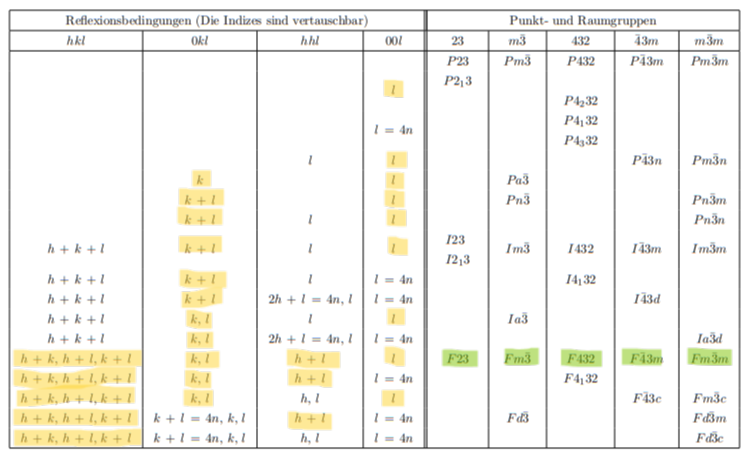
\includegraphics[angle = 90, width = 0.8 \linewidth]{Bilder/Auswertung/NaCl/table extinktion marked.png}
    \label{fig:reflexCond}
    \caption{For each of the reflex groups the fulfilled reflex conditions of the indexed peaks from tab.~\ref{tab:latticeParams} are marked in yellow. Subsequently, only a few point and space groups are left for the description of NaCl; they are marked in green. Table from~\cite{Aroyo2016}}
\end{figure}

Because further calculations would be far to complicated, we were hinted by the handout for the experiment, that the actual space group is $Fm\overline{3}m$. Remembering, that we found $Z=4$ and our structure is cubic, we assume, that NaCl is a face centered cubic (fcc) with a two atom basis (Na and Cl). Anyhow, we still do not know the basis. Therefore, two structure models $\mathbf{A}$ and $\mathbf{B}$ were suggested, where the coordinates of the atoms are $Na = (0\,0\,0)$, $Cl = (0.5\,0.5\,0.5)$ and $Na = (0\,0\,0)$, $Cl = (0.25\,0.25\,0.25)$, respectively. 